\documentclass[letterpaper,10pt,twoside,printwatermark=false]{pinp}

%% Some pieces required from the pandoc template
\providecommand{\tightlist}{%
  \setlength{\itemsep}{0pt}\setlength{\parskip}{0pt}}

% Use the lineno option to display guide line numbers if required.
% Note that the use of elements such as single-column equations
% may affect the guide line number alignment.

\usepackage[T1]{fontenc}
\usepackage[utf8]{inputenc}

% The geometry package layout settings need to be set here...
\geometry{layoutsize={0.95588\paperwidth,0.98864\paperheight},%
          layouthoffset=0.02206\paperwidth,%
		  layoutvoffset=0.00568\paperheight}

\definecolor{pinpblue}{HTML}{185FAF}  % imagecolorpicker on blue for new R logo
\definecolor{pnasbluetext}{RGB}{101,0,0} %



\title{Poll 1 - A Survey on Basic Statistics Concepts.}

\author[a]{EPIB607 - Inferential Statistics}

  \affil[a]{Fall 2018, McGill University}

\setcounter{secnumdepth}{5}

% Please give the surname of the lead author for the running footer
\leadauthor{Bhatnagar and Hanley}

% Keywords are not mandatory, but authors are strongly encouraged to provide them. If provided, please include two to five keywords, separated by the pipe symbol, e.g:
 \keywords{  Descriptive stats |  Confidence Interval |  p-value |  Gaussian distribution |  CLT |  Simple linear regression  }  

\begin{abstract}
This live poll was conducted on the first day of class, September 6,
2018. Correct answers are indicated by check marks. Number of votes and
number of participants are indicated in the figure legend. For some
questions, several selections were allowed.
\end{abstract}

\dates{This version was compiled on \today}
\doi{\url{https://sahirbhatnagar.com/EPIB607/}}

\pinpfootercontents{Poll 1 - September 6, 2018}

\begin{document}

% Optional adjustment to line up main text (after abstract) of first page with line numbers, when using both lineno and twocolumn options.
% You should only change this length when you've finalised the article contents.
\verticaladjustment{-2pt}

\maketitle
\thispagestyle{firststyle}
\ifthenelse{\boolean{shortarticle}}{\ifthenelse{\boolean{singlecolumn}}{\abscontentformatted}{\abscontent}}{}

% If your first paragraph (i.e. with the \dropcap) contains a list environment (quote, quotation, theorem, definition, enumerate, itemize...), the line after the list may have some extra indentation. If this is the case, add \parshape=0 to the end of the list environment.


\section{Which of the following visual summaries do you know about?
(select all that
apply)}\label{which-of-the-following-visual-summaries-do-you-know-about-select-all-that-apply}

\begin{enumerate}
\def\labelenumi{\arabic{enumi}.}
\tightlist
\item
  Histograms
\item
  Stem \& Leaf plots
\item
  Boxplot
\item
  Dotplot
\item
  Scatterplot
\item
  Density plot
\item
  Violin plot
\end{enumerate}

\begin{figure}[H]
  \begin{center}
    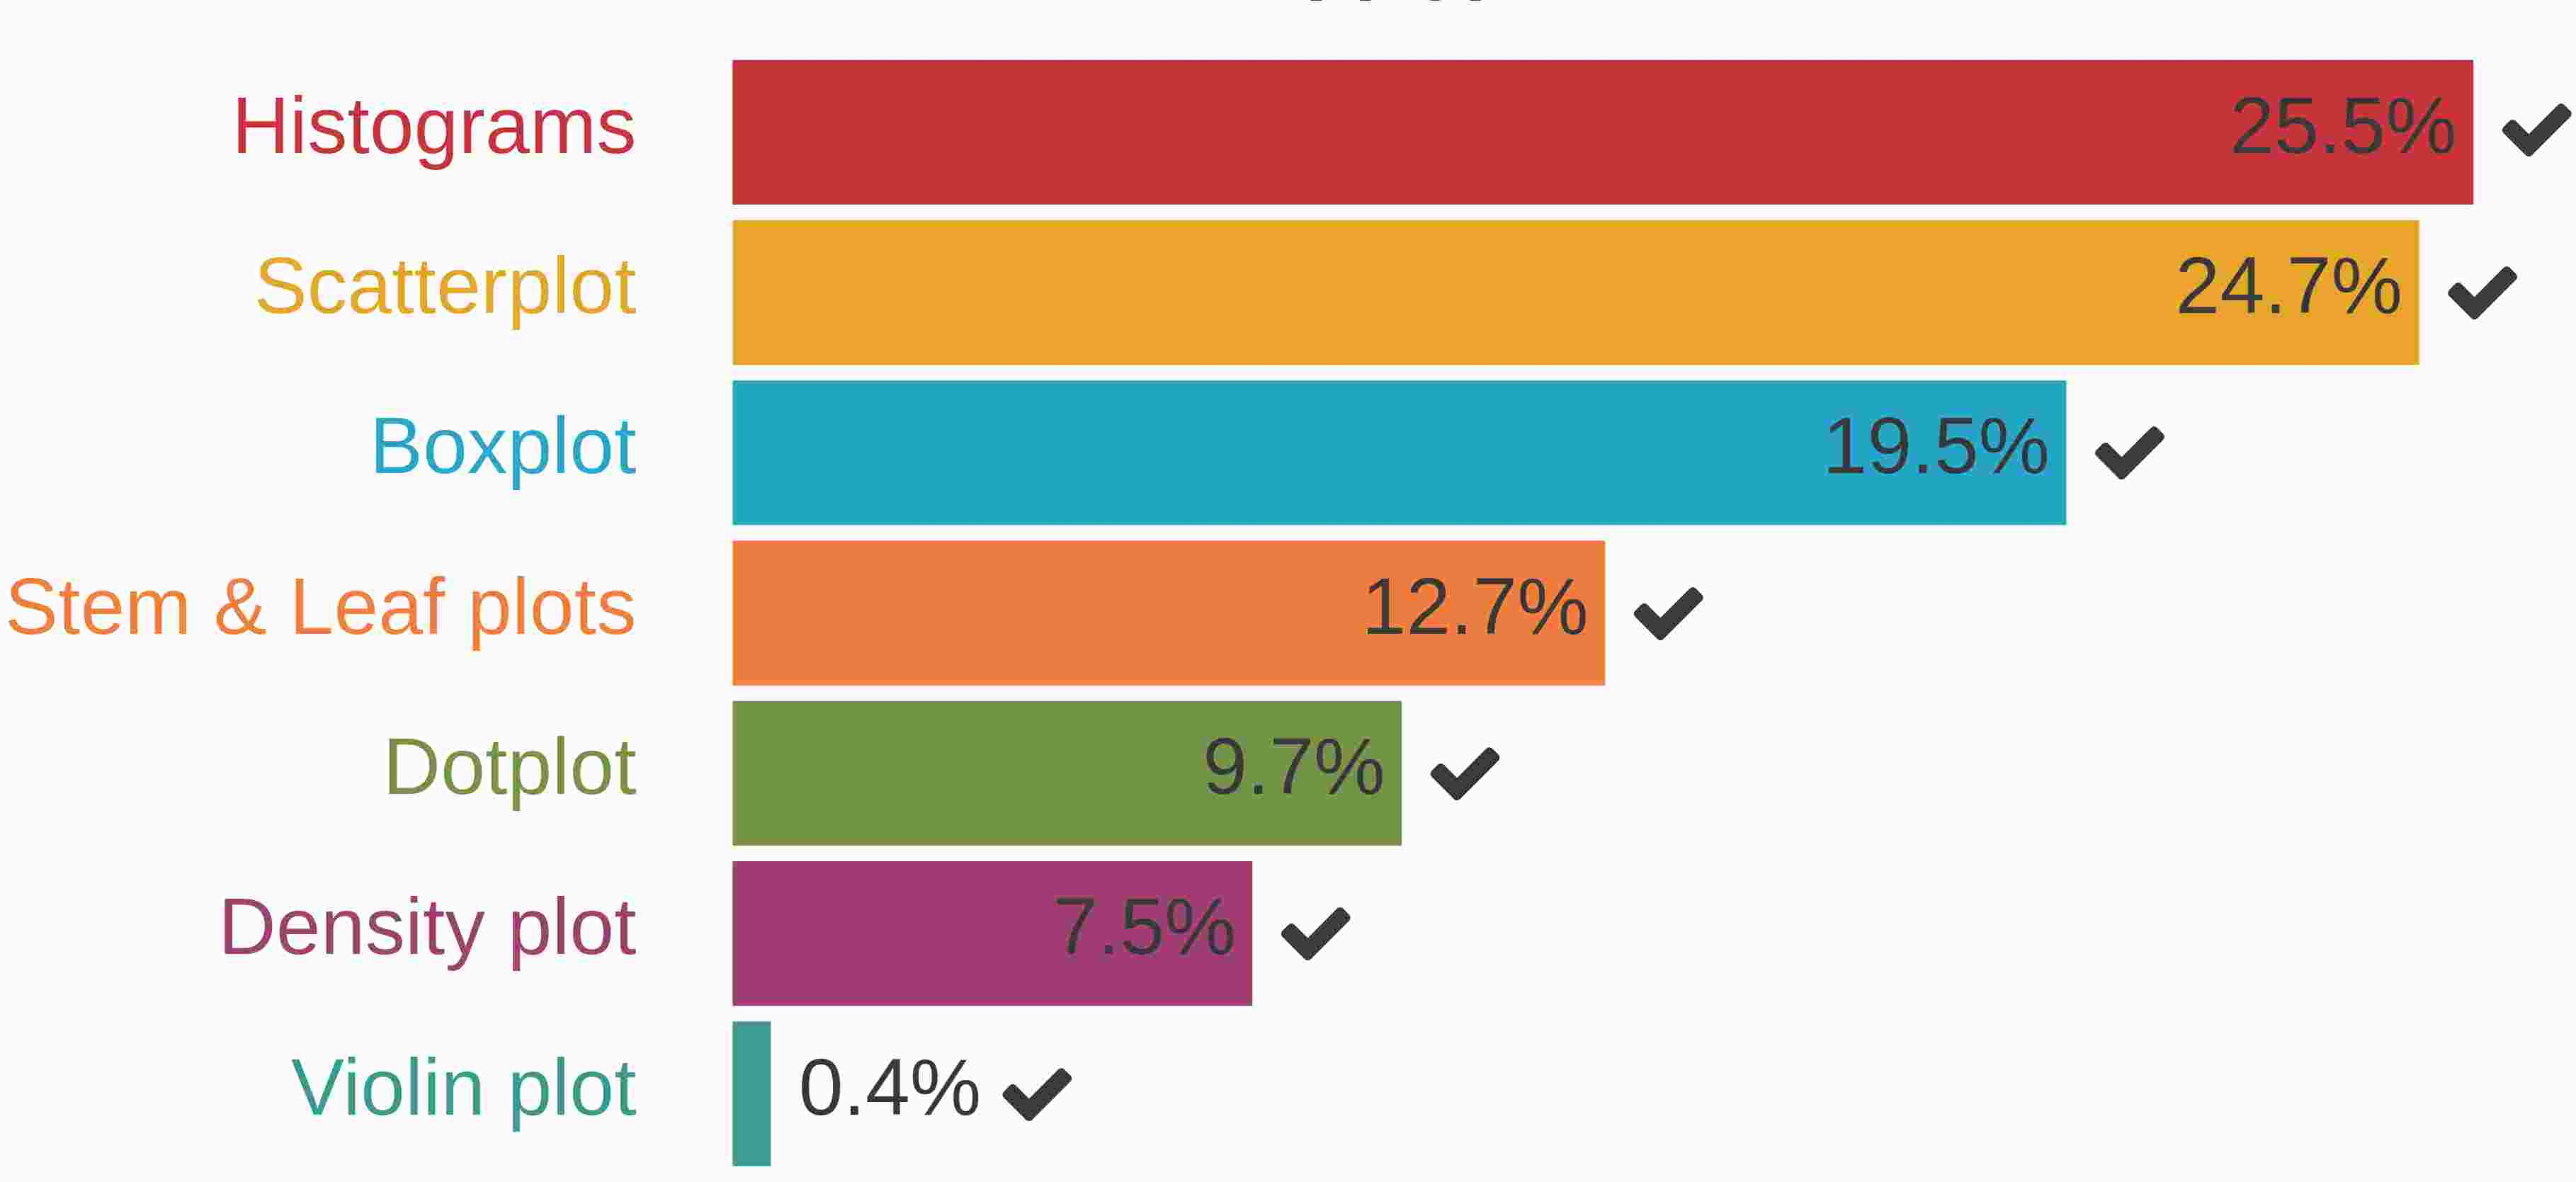
\includegraphics[scale=0.15]{q1.jpg} 
  \end{center}
  \caption{267 votes - 69 participants}\label{fig}
\end{figure}

\newpage

\section{A study records the sex and weight (in kilograms) of 30
recently born bear cubs in Alaska. Which of the following statements is
true?}\label{a-study-records-the-sex-and-weight-in-kilograms-of-30-recently-born-bear-cubs-in-alaska.-which-of-the-following-statements-is-true}

\begin{enumerate}
\def\labelenumi{\arabic{enumi}.}
\tightlist
\item
  Both are categorical variables
\item
  Both are quantitative variables
\item
  Sex is categorical, Weight is quantitative
\end{enumerate}

\begin{figure}[H]
  \begin{center}
    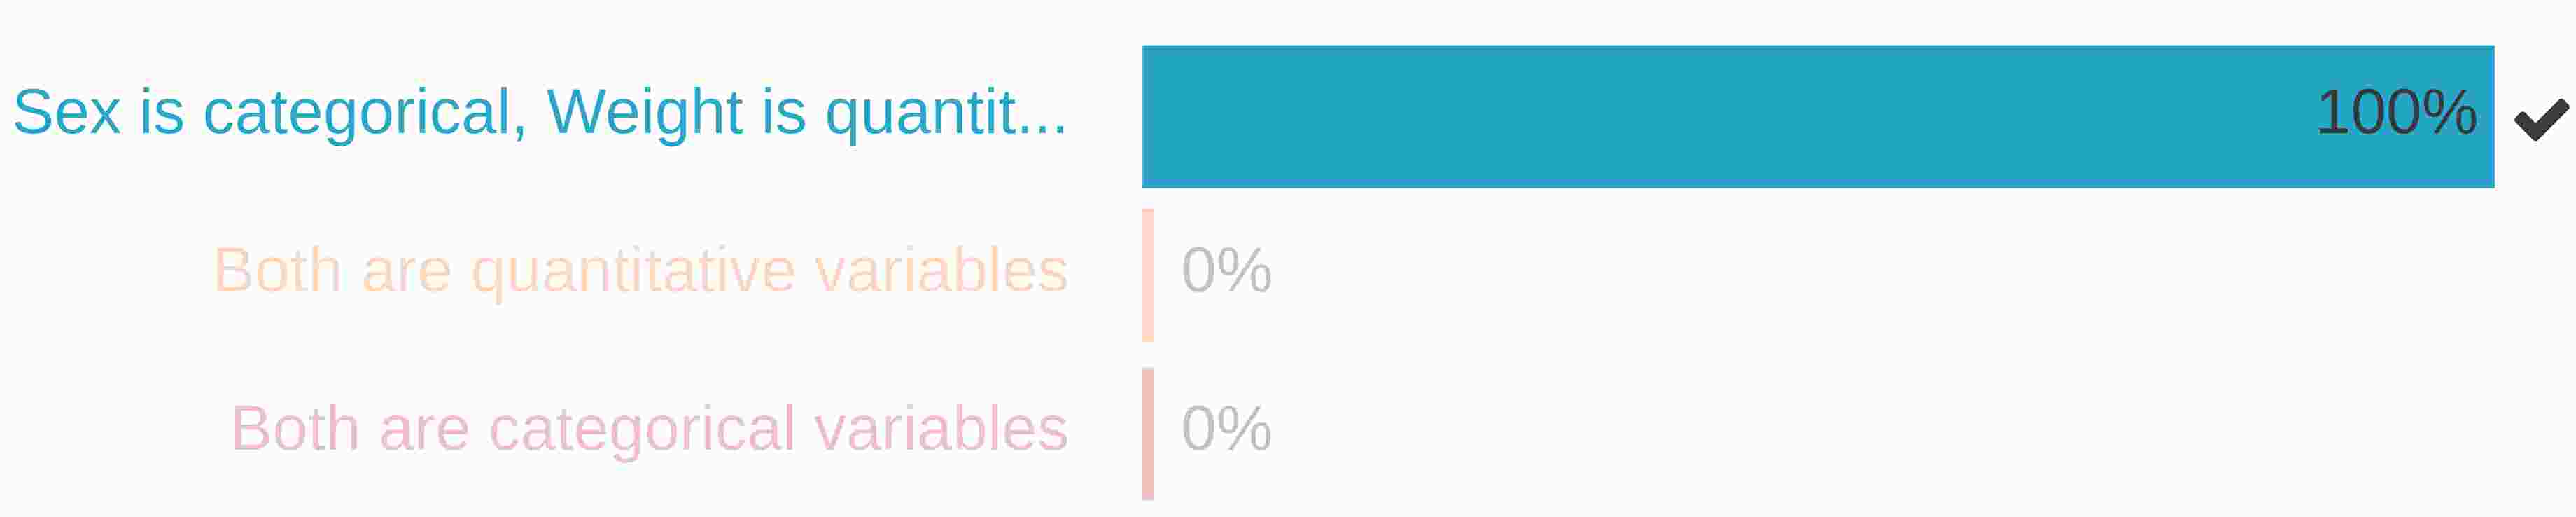
\includegraphics[scale=0.15]{q2.jpg} 
  \end{center}
  \caption{72 votes - 72 participants}
\end{figure}

\section{You are given a sequence of 5 numbers: 1, 5, 20, 35, 39. Which
of the following statements are
true?}\label{you-are-given-a-sequence-of-5-numbers-1-5-20-35-39.-which-of-the-following-statements-are-true}

\begin{enumerate}
\def\labelenumi{\arabic{enumi}.}
\tightlist
\item
  The median is equal to the mean
\item
  The median is less than the mean
\item
  The median is greater than the mean
\end{enumerate}

\begin{figure}[H]
  \begin{center}
    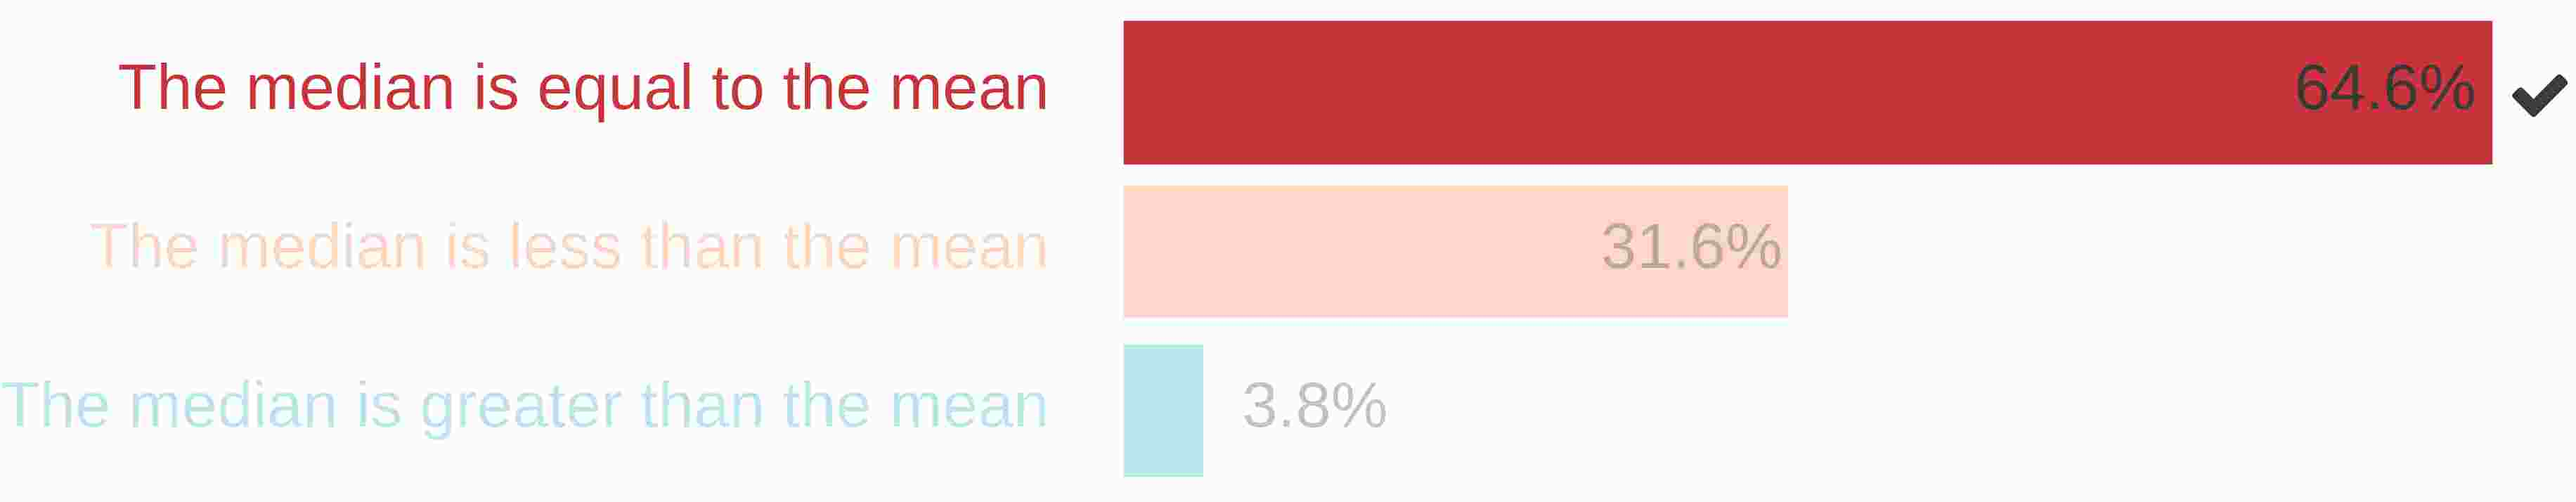
\includegraphics[scale=0.15]{q3.jpg} 
  \end{center}
  \caption{79 votes - 79 participants}
\end{figure}

\newpage

\section{In a distribution with a long right-tail, the median
is}\label{in-a-distribution-with-a-long-right-tail-the-median-is}

\begin{enumerate}
\def\labelenumi{\arabic{enumi}.}
\tightlist
\item
  equal to the mean
\item
  less than the mean
\item
  greater than the mean
\end{enumerate}

\begin{figure}[H]
  \begin{center}
    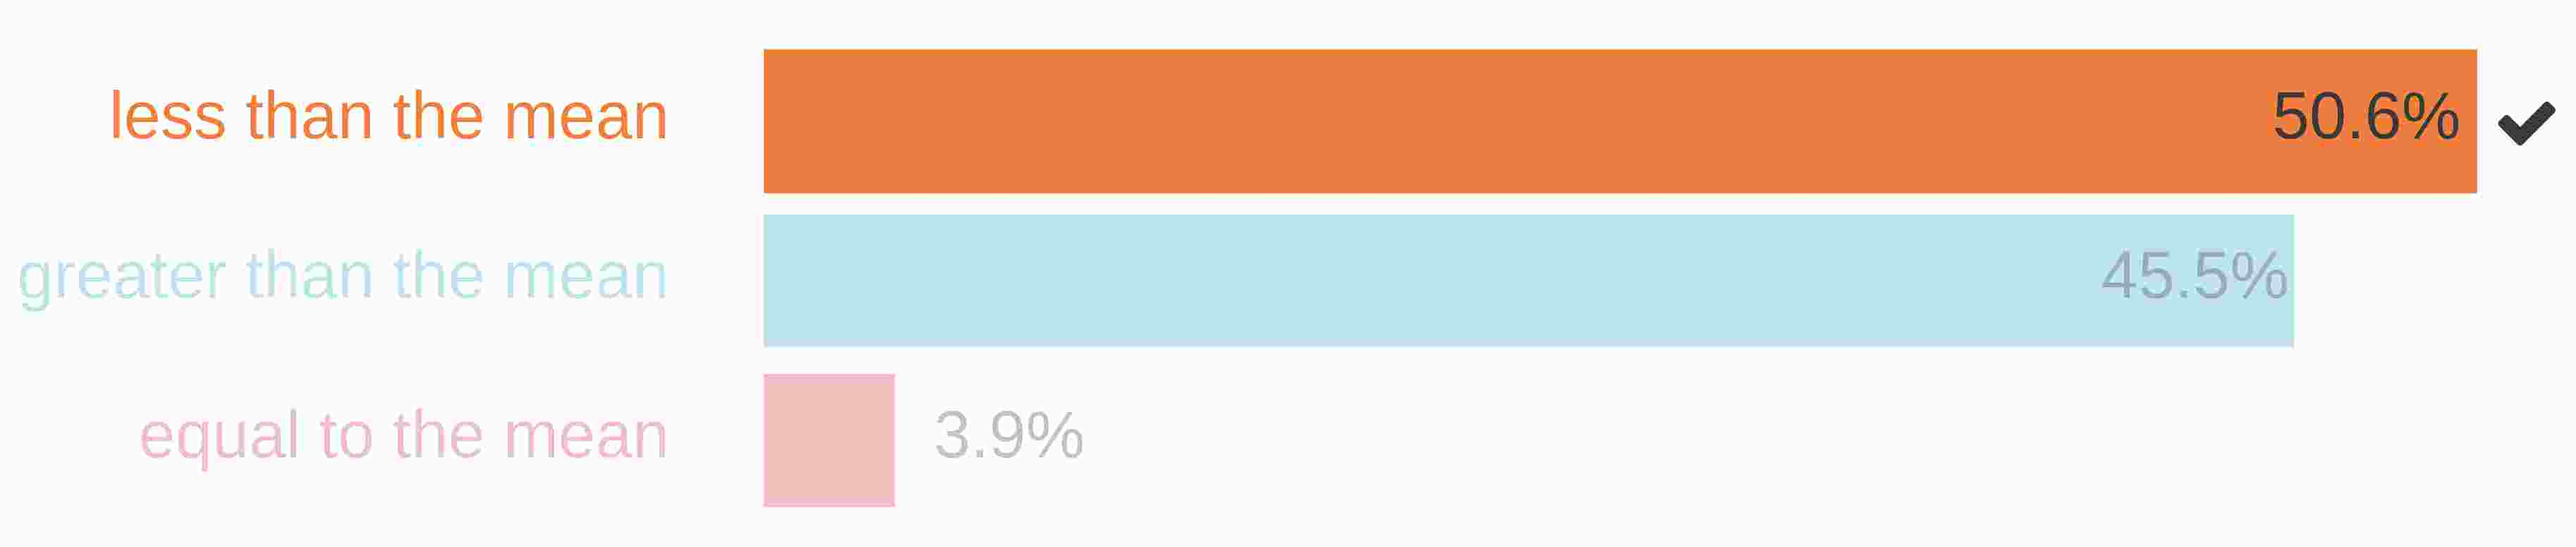
\includegraphics[scale=0.15]{q4.jpg} 
  \end{center}
  \caption{77 votes - 77 participants}
\end{figure}

\section{If you add 7 to each value on a sequence of numbers, the
standard deviation increases by
7}\label{if-you-add-7-to-each-value-on-a-sequence-of-numbers-the-standard-deviation-increases-by-7}

\begin{enumerate}
\def\labelenumi{\arabic{enumi}.}
\tightlist
\item
  TRUE
\item
  FALSE
\end{enumerate}

\begin{figure}[H]
  \begin{center}
    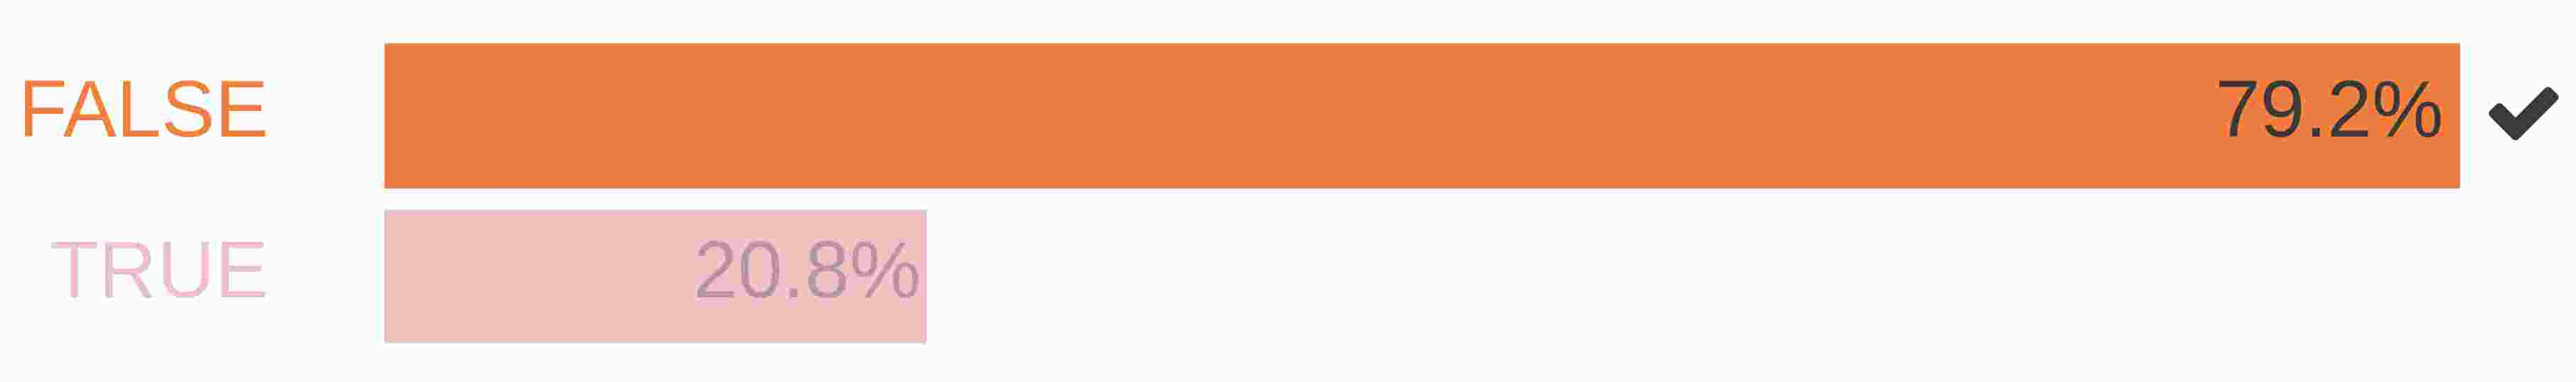
\includegraphics[scale=0.15]{q5.jpg} 
  \end{center}
  \caption{77 votes - 77 participants}
\end{figure}

\section{If you double each value on a sequence of numbers, you double
the standard
deviation.}\label{if-you-double-each-value-on-a-sequence-of-numbers-you-double-the-standard-deviation.}

\begin{enumerate}
\def\labelenumi{\arabic{enumi}.}
\tightlist
\item
  TRUE
\item
  FALSE
\end{enumerate}

\begin{figure}[H]
  \begin{center}
    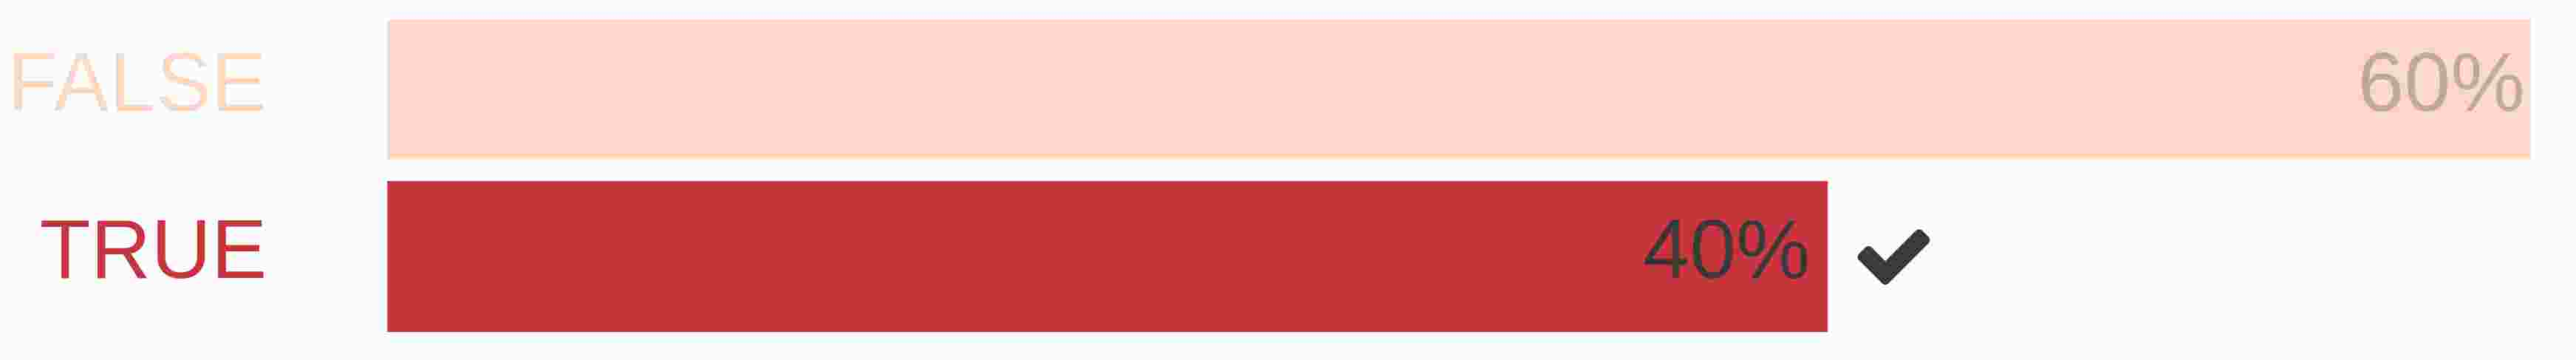
\includegraphics[scale=0.15]{q6.jpg} 
  \end{center}
  \caption{75 votes - 75 participants}
\end{figure}

\newpage

\section{In a large set of observations, the distribution of
observations follows the Gaussian curve quite
closely}\label{in-a-large-set-of-observations-the-distribution-of-observations-follows-the-gaussian-curve-quite-closely}

\begin{enumerate}
\def\labelenumi{\arabic{enumi}.}
\tightlist
\item
  TRUE
\item
  FALSE
\end{enumerate}

\begin{figure}[H]
  \begin{center}
    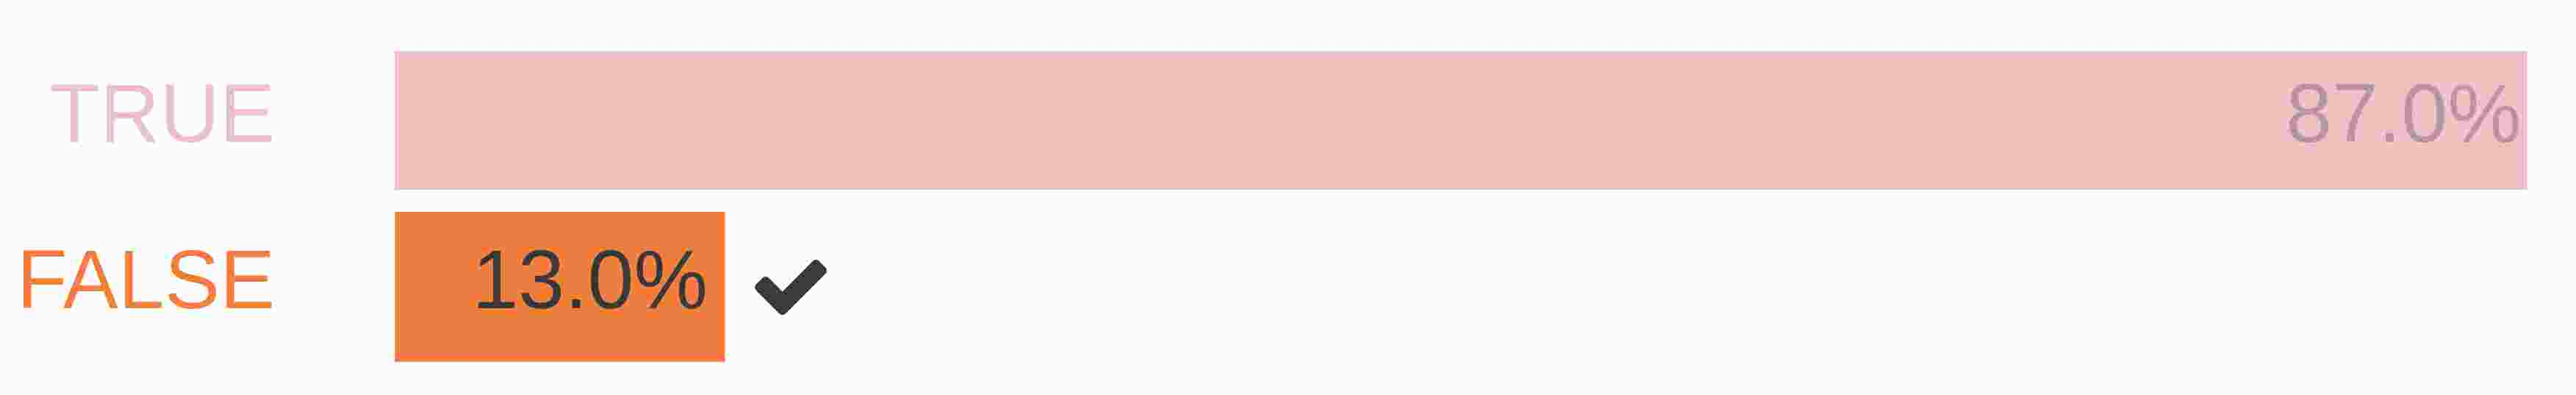
\includegraphics[scale=0.15]{q7.jpg} 
  \end{center}
  \caption{77 votes - 77 participants}
\end{figure}

\section{A straight line relating a response variable y to an
explanatory variable x is given by y = a + bx. Which of the following
statements are true? (select all that
apply)}\label{a-straight-line-relating-a-response-variable-y-to-an-explanatory-variable-x-is-given-by-y-a-bx.-which-of-the-following-statements-are-true-select-all-that-apply}

\begin{enumerate}
\def\labelenumi{\arabic{enumi}.}
\tightlist
\item
  b is the intercept and a is the slope
\item
  b is the slope and a is the intercept
\item
  the intercept a is the value of y when x=0
\end{enumerate}

\begin{figure}[H]
  \begin{center}
    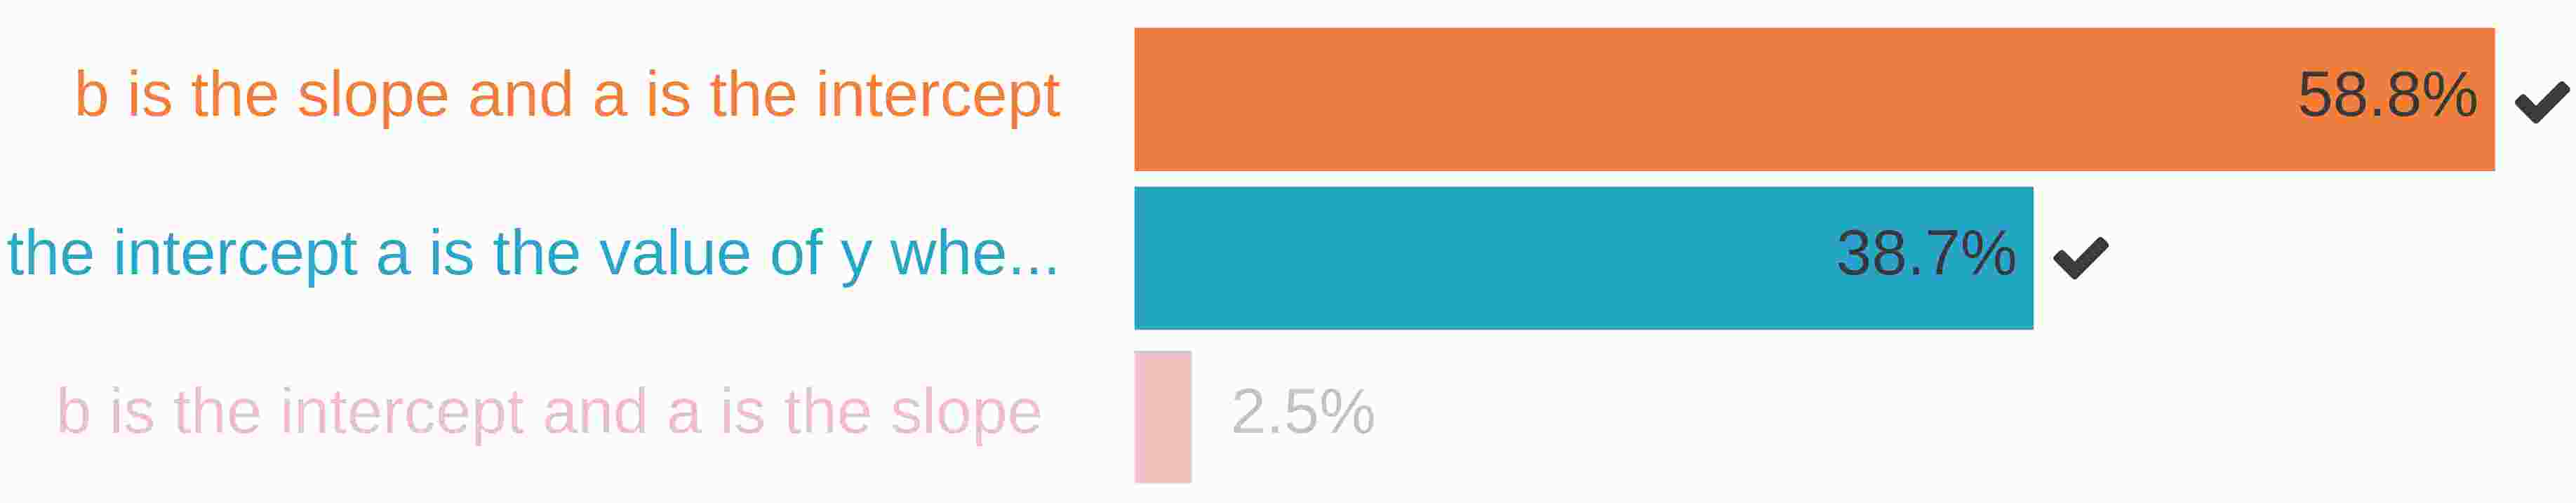
\includegraphics[scale=0.15]{q8.jpg} 
  \end{center}
  \caption{119 votes - 79 participants}
\end{figure}

\newpage

\section{A p-value is (select all that
apply)}\label{a-p-value-is-select-all-that-apply}

\begin{enumerate}
\def\labelenumi{\arabic{enumi}.}
\tightlist
\item
  conditional on the null hypothesis being true
\item
  a measure of evidence
\item
  the probability of the null hypothesis being true
\item
  a probability concerning the observed data
\item
  significant if it is less than 0.05
\item
  a probability that provides the same information as a confidence
  interval
\end{enumerate}

\begin{figure}[H]
  \begin{center}
    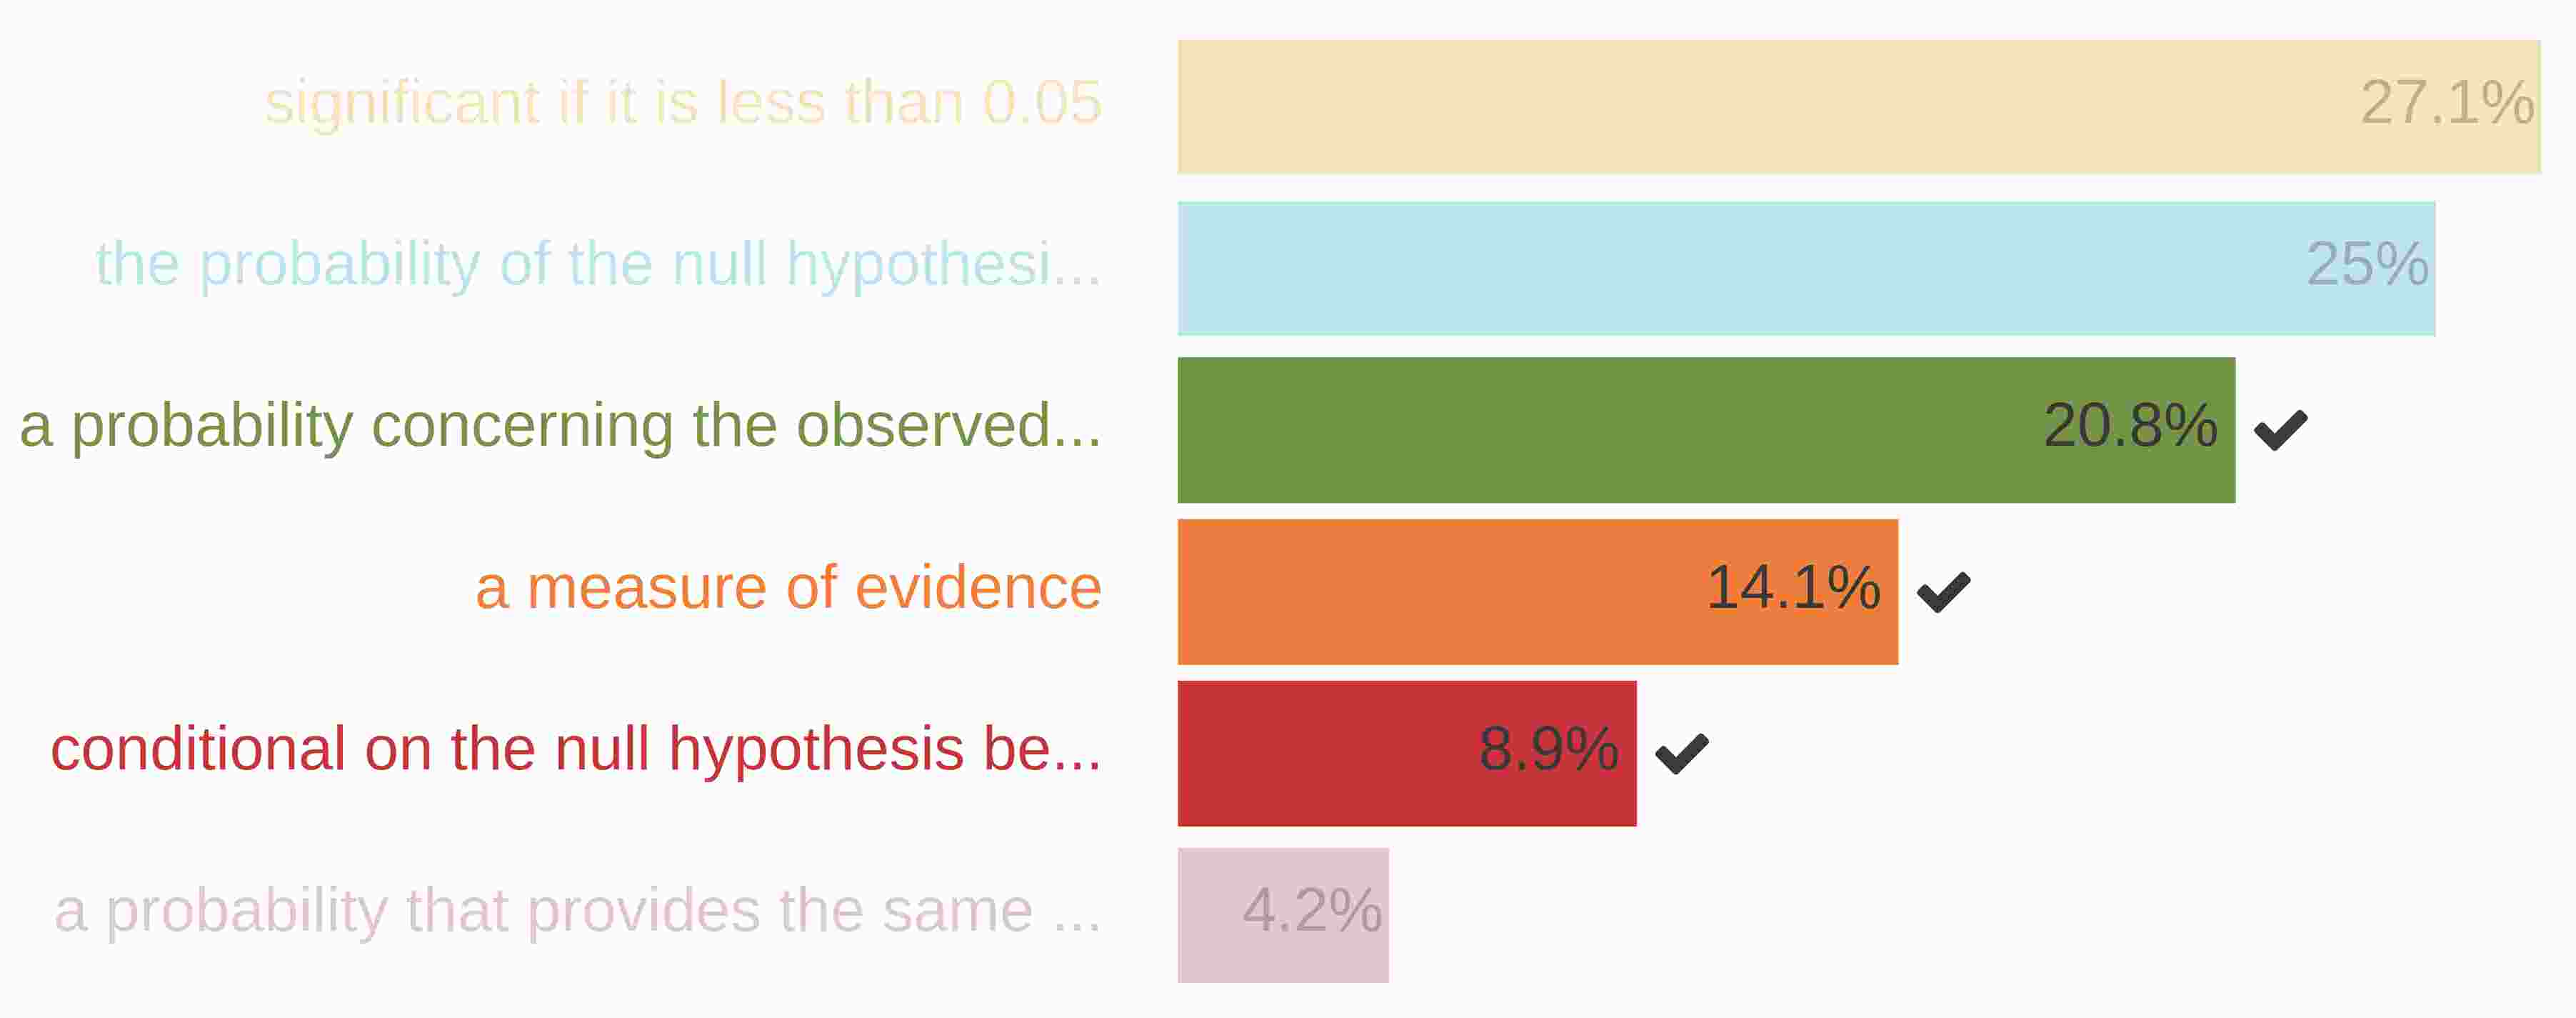
\includegraphics[scale=0.11]{q9.jpg} 
  \end{center}
  \caption{192 votes - 80 participants}
\end{figure}

\section{Which of the following statements are correct regarding a
confidence interval? (select all that
apply)}\label{which-of-the-following-statements-are-correct-regarding-a-confidence-interval-select-all-that-apply}

\begin{enumerate}
\def\labelenumi{\arabic{enumi}.}
\tightlist
\item
  It often has the form: estimate +/- margin of error
\item
  Is an interval estimate computed from sample data that gives a range
  of plausible values for a population parameter
\item
  The interval is constructed so that the value of the parameter will be
  captured between the endpoints of the interval with a chosen level of
  confidence
\item
  The confidence level is the success rate for the method
\item
  provides more useful information than the p-value
\end{enumerate}

\begin{figure}[H]
  \begin{center}
    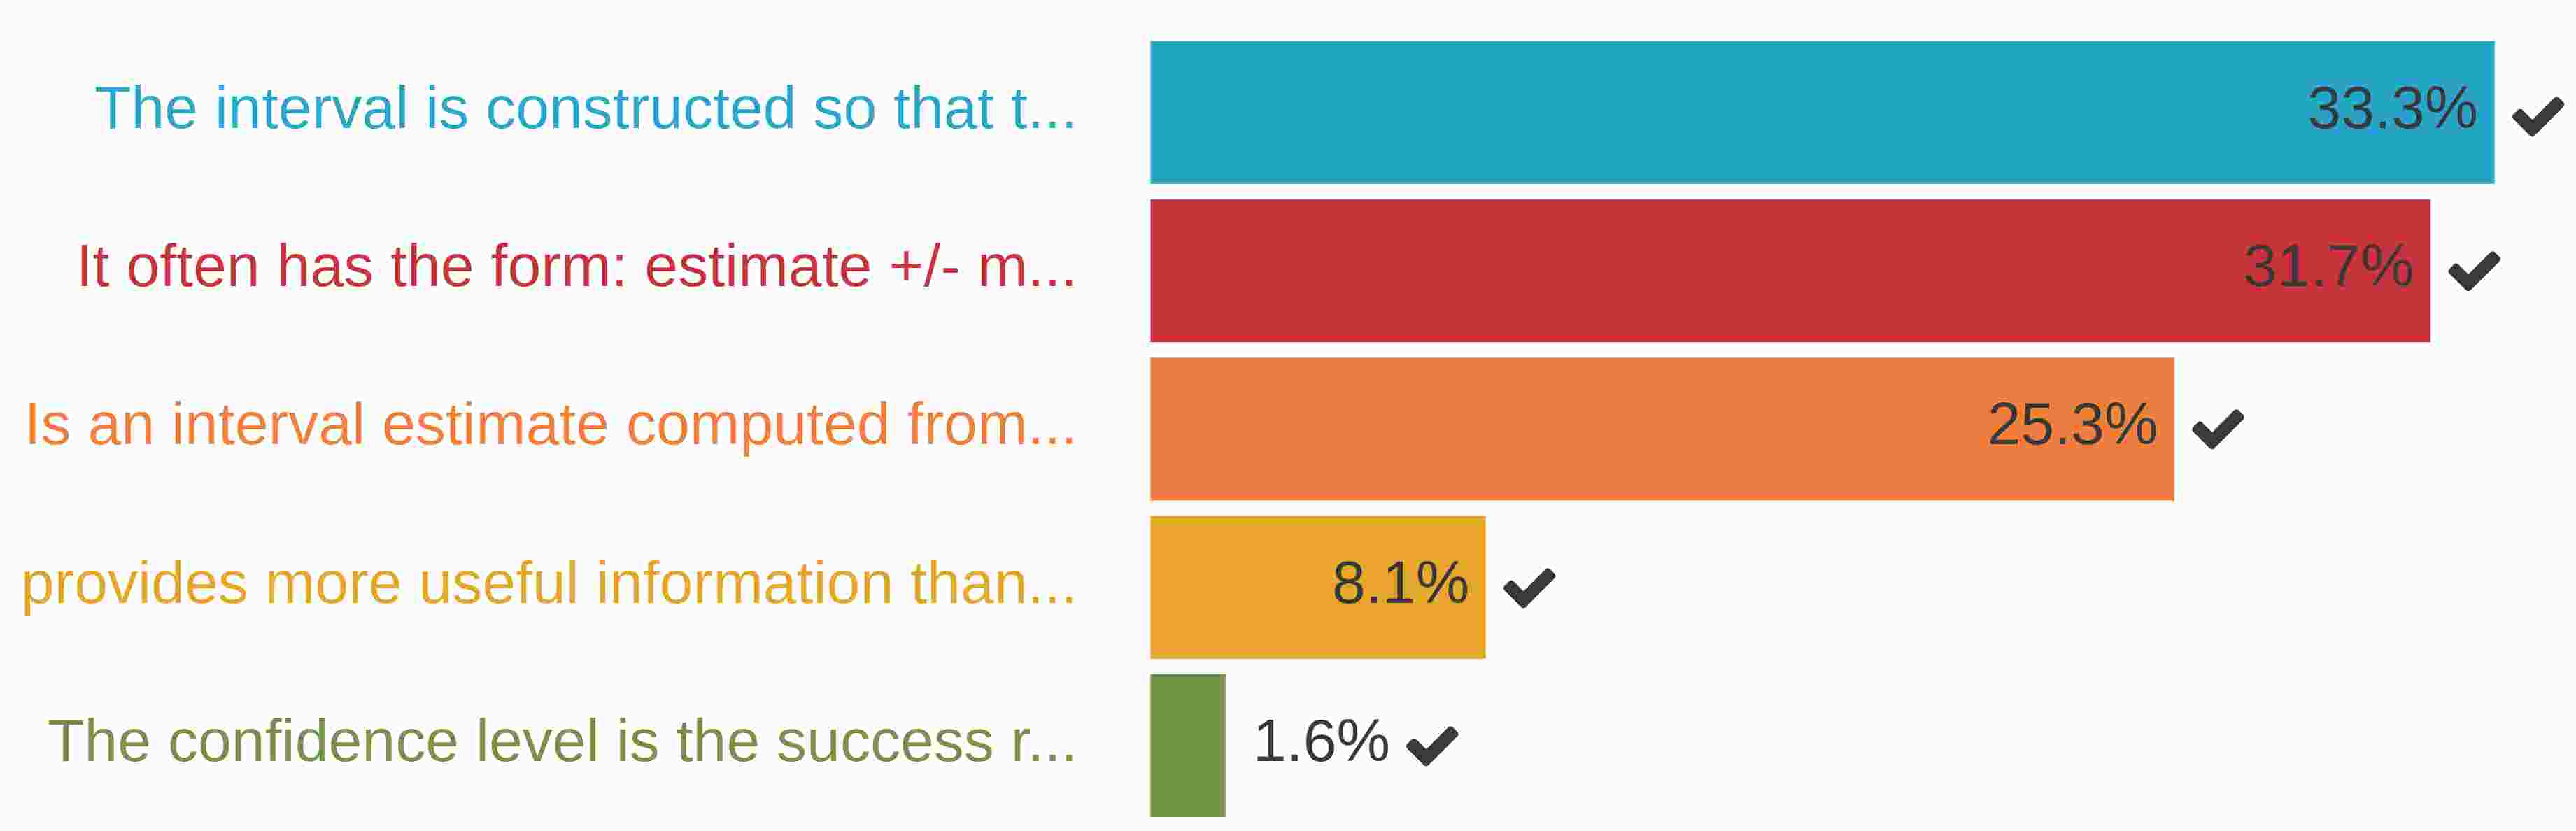
\includegraphics[scale=0.11]{q10.jpg} 
  \end{center}
  \caption{186 votes - 79 participants}
\end{figure}

%\showmatmethods


\bibliography{pinp}
\bibliographystyle{jss}



\end{document}

